\cleardoublepage

\chapter{Especificación del protocolo blockchain}
\label{cap3}
Una vez se han visto las dos nociones criptográficas fundamentales en las que se fundamenta el blockchain (algoritmo ECDSA y funciones Hash) es posible explicar tanto el funcionamiento de este protocolo como justificar su corrección. 
Aunque las ideas fundamentales que serán expuestas están basadas en el artículo original del Bitcoin \citep{bitcoin} en los puntos en los que existan divergencias entre distintas implementaciones del protocolo se intentarán señalar las diferentes alternativas. Siendo esta una tecnología que se ha desarrollado más con la práctica a través de diversas implementaciones que con trabajos teóricos resulta complicado abarcar en un solo trabajo todas sus variantes.

\section{Objetivos del Blockchain}\label{objetivos}
El Bitcoin surgió con el objetivo de por un lado eliminar la necesidad  de una entidad de confianza que actúe de intermediario en las transacciones económicas digitales y por otro lado de resolver el problema derivado de la ausencia de este ente \citep{bitcoin}. En un intercambio basado en artículos físicos a los que se le asigna cierto valor (el papel moneda por ejemplo) los únicos problemas de los que las partes deben preocuparse son aquellos derivados de la estafa o la falsificación. Cuando estas transacciones se realizan sin intervenir medios físicos no se puede garantizar que la parte encargada de entregarle la retribución monetaria a la otra posea los medios económicos que dice tener. Más aún, alguien aún disponiendo de la capacidad de realizar cierta transacción puede enviarle a diferentes individuos cantidades que por separado no superen sus fondos, pero que en conjunto sí lo hagan, este es el llamado problema del doble gasto. Los intermediarios cumplen entonces la función de evitar que esto ocurre al llevar un registro actualizado de las transacciones de cada cliente y por tanto de los fondos de los que dispone.

Pero, ¿qué sentido tiene entonces eliminar el intermediario si con ello solo generamos problemas que debemos resolver? Un sistema descentralizado tolera mucho mejor las particiones que uno centralizado: basta aislar al servidor para dejar inoperativa toda la red. Además, desde el punto de vista de la seguridad cualquier ataque con éxito al servidor supone a su vez la caída de todo el sistema. Incluso suponiendo que se dispone de un intermediario seguro y distribuido en diferentes nodos de forma que la caída de alguno de ellos no suponga mayor problema para la red, la pregunta que debemos hacernos es cuanto podemos llegar a confiar en esta entidad. En la medida en que controla nuestro dinero puede llegar a actuar de forma más o menos arbitraria con él ya sea por interés propio o al servicio de algún poder externo. Ejemplos en la vida real hay muchos.

El objetivo será por tanto proporcionar un protocolo seguro, que aún estando completamente descentralizado pueda resolver en particular el problema del doble gasto y en general problemas de consenso de otra clase. Por tanto, la corrección de este protocolo vendrá dada por la comprobación de que justamente se han solucionado estas cuestiones.
%Como se mencionó en la introducción, el blockchain consiste en esencia en un registro distribuido e inmutable

\section{Configuración de la red}
El protocolo Blockchain se define e implementa sobre una red basada en la arquitectura peer-to-peer (red entre pares). El término peer-to-peer (en lo adelante P2P) viene a decir que al contrario que en un sistema cliente/servidor aquí todos los nodos realizan potencialmente las mismas funciones. Este punto puede no ser del todo cierto en determinadas implementaciones como por ejemplo en Blockchain de consorcio o privados, pero en estos casos es el protocolo elegido y no la estructura de la red quien restringe las funciones de algunos nodos. Estas restricciones no limitan en ningún caso la capacidad de enviar o recibir información directamente entre los participantes, sino que está controlada que clase de información determinados nodos pueden enviar y como los demás interpretan estos mensajes. El Bitcoin es el ejemplo más importante de red blockchain donde no hay ninguna clase de jerarquía 

Aunque todos los nodos teóricamente puedan realizar las mismas funciones en la práctica suelen elegir que tareas realizar y cuales ignorar. Así, algunas máquinas pueden dedicarse a ejecutar las labores más complejas del algoritmo de consenso (más adelante veremos en que consiste este algoritmo), otras  almacenan parte (o la totalidad) de la cadena de bloque, mientras que otros nodos ejecutan tareas de verificación. Existen otras especializaciones (o combinaciones de especializaciones) que pueden variar entre diferentes implementaciones del blockchain.

%La información transmitida desde un punto en una red P2P debe alcanzar a casi todos los nodos, extenderse algo más aquí.
Un problema importante en las redes es P2P es como los participantes se encuentran unos con otros para establecer una conexión. Los nodos mantienen un registro privado de las direcciones IP con las que se han comunicado, y pueden compartir este registro con otros miembros que lo soliciten, esta sería la forma estándar de ampliar la agenda de contactos. La primera vez que un nodo se une a la red dispone de una lista de direcciones IP prefijada, además, en ciertos protocolos blockchain que han alcanzado un número de participantes considerable existe también la posibilidad de conectarse a varias DNS \textit{Seed} (DNS son las siglas de \textit{Domain Name System}) donde se recibe una lista generada aleatoriamente de otros nodos que han estado activos en la red en un rango de tiempo determinado. Los servidores DNS sirven para asociar direcciones IP con nombres de dominio, en el caso del protocolo blockchain en general y del Bitcoin en particular, las direcciones IP almacenadas se corresponden con nodos de la red. Este punto, dado que es el único en el que existe algo de centralización, entraña ciertos riesgos, pues alguno de estos DNS \textit{Seed} puede caer bajo el control de una entidad maliciosa que le proporcione a los nuevos participantes solo direcciones ip de nodos bajo su control, de esta forma se podría crear una red independiente de la principal donde existe una cadena de bloques generada de forma arbitraria. Por ello se mantiene cierto control de forma pública y abierta sobre estas DNS \textit{Seed} y se puede igualmente usar direcciones IP  recibidas a través de cualquier otra vía.


\section{Cadena de bloques}\label{bloques}
El componente fundamental del blockchain es la estructura de datos donde se almacena toda la información que los nodos que participan en el protocolo han acordado que es válida. En las criptomonedas este registro cumple la función de libro de cuentas, sin embargo, se pueden guardar todo tipo de datos.

Cada uno de los bloques que conforman esta cadena además de la propia información que pueda contener mantiene una referencia al bloque anterior. La excepción a esto es el bloque inicial, que se genera de forma diferente al resto.
Esta estructura enlazada no es suficiente para garantizar la integridad de la cadena de bloques, pues un adversario podría modificar la información almacenada en un bloque dejando intacta la referencia al bloque anterior. Aquí es donde se utilizan por primera vez las funciones hash definidas en \ref{hash}: además de la información almacenada y la referencia al bloque anterior guardaremos también el resultado de aplicar cierta función hash al conjunto de los datos del bloque (incluido quien es el bloque anterior). Si la función elegida es resistente frente a segundas preimágenes se puede verificar que  el bloque es correcto simplemente aplicándole la función Hash a sus datos y comparando con la almacenada. Y la referencia al bloque anterior en lugar de ser únicamente un índice incluirá también el valor hash de ese bloque.

Sin embargo, aún con este añadido seguimos sin tener garantizado que un adversario pueda hacer modificaciones en la cadena. Es cierto que ahora para hacer cambios en un único bloque tendría que generar nuevamente toda la cadena a partir de ese bloque, pero el coste de operar con funciones hash es lineal, así que es factible hacer estas modificaciones en un tiempo razonable. Además de la referencia al bloque anterior y la información del bloque actual en los datos que sobre los que se aplica la función hash se incluirá un valor generado de forma aleatoria, así se garantiza que la cadena hash resultante tenga ciertas propiedades definidas en el protocolo. Por ejemplo, en el Bitcoin a la cadena hash se le pide que comience por cierto número de ceros. El cálculo de este valor aleatorio, denominado nonce (number used once), es la tarea principal del algoritmo de prueba de trabajo que se verá en el siguiente apartado.

Otra información que se incluye en los bloques, asociada con la función hash, es una marca temporal (\textit{timestamp}) del momento en que fue creado el bloque. De esta forma se puede probar que la información existía cuando se calculó el valor hash. Mantener un registro temporal también servirá en el algoritmo de consenso para rechazar directamente aquellos bloques con marcas de tiempo superiores al momento actual.

Por último, y con el objetivo de reducir el uso de espacio, el conjunto de operaciones almacenadas en un bloque no se guardan explícitamente. En su lugar se almacena la raíz del árbol Merkle resultante. En la siguiente sección esta estructura de datos será analizada.

Lo anterior se puede considerar más o menos estándar en todas las implementaciones del blockchain, pero se pueden incluir otros elementos dentro de cada bloque.
\begin{figure}[H]
%\centering
  \subfloat[Diagrama Blockchain (Fuente \url{http://www.doc.ic.ac.uk/~ma7614/topics_website/tech.html}
)]%
  {{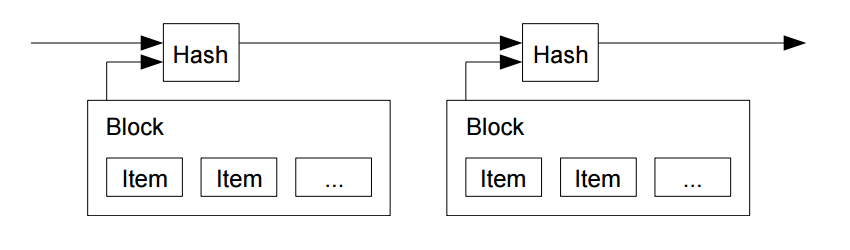
\includegraphics[width=12cm]{figures/blockchain_diagram.png}}}%
  \qquad

	\label{fig:blockchain}%
\end{figure}

\section{Árboles Merkle}\label{merkle}
Los árboles Merkle, patentados en 1979 por Ralph Merkle\citep{merkle1987digital} han sido usados activamente en la verificación de bases de datos.
En el caso del Blockchain para cada transacción se calcula su valor hash, combinando estos resultados en pares se reduce a la mitad el número de valores que hay que almacenar. Repitiendo este proceso, ahora para los valores resultantes se llega a un valor hash final, llamado raíz hash, que se ha calculado de forma determinística a partir de los valores originales (transacciones).

Por ejemplo, si se desean guardar las transacciones A,B,C,D en cierto nodo calculamos en primer lugar, H(A), H(B), H(C), H(D) donde H es la función hash que estemos utilizando. Posteriormente se calcula H((H(A),H(B) y H(H(C),H(D)), por último queda aplicarle la función H a estos dos valores, y se tiene entonces la raíz Merkle que se incluirá en el bloque.

Por las propiedades de las funciones hash vistas antes, se garantiza la integridad de las transacciones almacenadas, pues cualquier ligera modificación en las mismas produciría cambios en la raíz Merkle resultante y por tanto ese bloque se rechazaría. Ademas, la propia estructura de los arboles Merkle nos permite encontrar que transacción ha cambiado, pues basta descender desde la raíz comparando cada uno de los valores hash almacenados hasta encontrar la transacción, que viene a ser una hoja del árbol, que ha sido modificada.

Los árboles Merkle permiten de esta forma hacer verificaciones sobre el estado de la cadena de forma rápida y permitiendo un menor uso de almacenamiento.

\begin{figure}[H]
\centering
  \subfloat[Diagrama Árbol Merkle (Fuente \url{https://www.researchgate.net/publication/324385574_Towards_Decentralized_Accountability_and_Self-sovereignty_in_Healthcare_Systems}]{{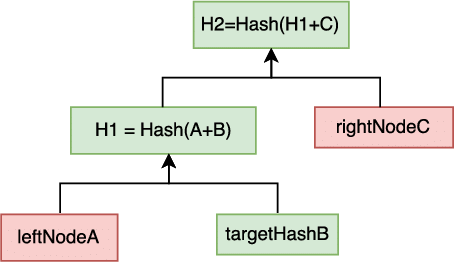
\includegraphics[width=12cm]{figures/merkle_tree.png}}}%
  \qquad

	\label{fig:merkle}%
\end{figure}


\section{Algoritmo de prueba de trabajo}\label{chap3:pow}
La estructura en cadena de bloques enlazados usando funciones hash no resuelve por si sola el problema del doble gasto visto en \ref{objetivos}, para eso hay que establecer un algoritmo que permita a los participantes decidir que información se puede incluir en la cadena de bloques, validando de esta forma las transacciones correctas. En el Bitcoin se estableció como tal sistema el algoritmo de prueba de trabajo (Proof of Work) \citep{bitcoin}, en posteriores implementaciones del Blockchain, salvo ciertas modificaciones se ha mantenido en general este mismo algoritmo. La idea de la prueba de trabajo se originó para resolver el problema del uso abusivo de ciertos recursos como el correo electrónico mediante el envío masivo de mensajes de spam. Hashcash \citep{hashcash}, una de las primeras implementaciones de un mecanismo para solucionar este problema, se basaba en usar una función de coste para generar una ficha que permitiría disponer de cierto recurso. Esta ficha probaba que el usuario había invertido determinado tiempo de procesamiento en resolver el problema planteado por la función de coste y de esta forma el uso del recurso en cuestión estaba condicionado por la resolución de cierto problema que conllevaba determinado uso de CPU por parte del usuario. Con el Bitcoin este planteamiento basado en un sistema cliente-servidor fue extendido a un contexto descentralizado.

El resultado de ejecutar la función de coste (ficha) debe poder ser verificado fácilmente por cualquiera, mientras que el cálculo de esta función debe ser una tarea moderadamente complicada. La funciones hash cumplen estos requisitos y son usadas como función de coste. Un participante que quiera validar un bloque, es decir, que quiera afirmar que cierto conjunto de transacciones o datos son válidos y que por tanto se pueden añadir al registro toma el bloque tal y como se definió en \ref{bloques} le añade cierto valor en bits cuya posible longitud y posición dentro del bloque están determinados en el protocolo y analiza el resultado de aplicarle cierta función hash acordada. Si este resultado cumple ciertos requisitos (por ejemplo la cadena hash devuelta empieza por cierto número de \textit{ceros}) entonces se dice que se ha resuelto el problema del algoritmo de prueba de trabajo (llamado puzzle en algunas fuentes) y se comparte con los demás nodos este resultado. Puede encontrarse también en ciertos artículos y especificaciones de criptomonedas que el puzzle que se debe resolver para validar cierto bloque consiste en encontrar una cadena hash menor que cierta longitud. Esto no es más que buscar cadenas hash que comiencen con ciertos número de ceros y considerarlas como de tipo numérico donde esos ceros desaparecen dejando una cadena $n$ posiciones más corta que la longitud hash de la función del algoritmo. 

En el algoritmo \ref{alg:pow} se presenta una posible especificación (muy simplificada) del método de prueba de trabajo para calcular un \textit{nonce} asociado a cierto bloque. En esta especificación se supone que quien la ejecuta ha verificado antes que todas los datos que se pretenden incluir en la cadena son correctos. Este algoritmo tal y como está planteado puede no terminar, pues es posible que no exista ningún \textit{nonce} de longitud menor o igual que $m$ que resuelva el puzzle. En la práctica si el bloque $b$ está formado por cadenas de la forma $b = s+p+k+t_{1}+ \ldots + t_{q}$ donde $s$ es el \textit{timestamp}, $p$ la referencia al valor hash del bloque anterior, $k$ es la clave pública del nodo que está calculando el \textit{nonce} y $t_{i}$ el conjunto de datos que almacena el bloque, se suele proceder reordenando los $t_{i}$ a la vez que se modifica el \textit{nonce} y comprobando el resultado de estas combinaciones. También se suelen hacer pequeñas modificaciones en el \textit{timestamp} $s$, pues entre la hora marcada por el bloque anterior y lo que se tarda en generar el siguiente bloque hay un rango de tiempo en el que moverse. Este proceso es lo que se conoce en las criptomonedas como minado. Las implementaciones de este algoritmo deben incluir, una condición de parada extra, pues no tiene sentido seguir operando si alguien ya ha resuelto el puzzle, así, se debe mantener un proceso que en caso de recibir información sobre la resolución (correcta) del problema de prueba de trabajo para el bloque en el que se está trabajando detenga el algoritmo. 

\begin{algorithm}
\caption{Prueba de trabajo (Cálculo)}\label{alg:pow}
\begin{algorithmic}[1]
\Require \Statex $H$ función hash del protocolo de longitud de cadena $k$.\Statex $l$ < $k$ longitud (dificultad) del puzzle.\Statex $m$ longitud máxima del nonce.\Statex $b$ bloque que se quiere validar.
\State Generar \textit{nonce} de forma aleatoria tal que $|nonce| \leq m$ \label{alg:pow:step1}
\If{$|H(nonce+b)| \leq l$} \Return $(nonce, b)$
\Else  Volver a  \ref{alg:pow:step1}
\EndIf
\end{algorithmic}
\end{algorithm}

Se incluye también el algoritmo de verificación que deben utilizar los nodos para comprobar el par $(nonce, b)$. Si acepta el bloque la forma de comunicarlo al resto de la red es incluir ese bloque en la cadena y empezar a trabajar en uno nuevo que lo tenga como predecesor. Puede ocurrir que diferentes nodos acepten distintos bloques en determinado punto, esto se denomina bifurcación y se trata en la siguiente sección.
\begin{algorithm}
\caption{Verificación de la prueba de trabajo}\label{alg:pow_check}
\begin{algorithmic}[1]
\Require \Statex $H$ función hash del protocolo de longitud de cadena $k$.\Statex $l$ < $k$ longitud (dificultad) del puzzle.\Statex $m$ longitud máxima del nonce. \Statex $(nonce, b)$
\State Se comprueba que $b$ está formado por datos válidos (bloque previo, timestamp y transacciones). Si falla cualquiera de estas comprobaciones \textbf{rechazar}
\If{$|H(nonce+b)| \leq l$} \Return \textbf{aceptar el bloque}
\Else  \textbf{ rechazar}
\EndIf
\end{algorithmic}
\end{algorithm}

\begin{figure}[H]
%\centering
  \subfloat[Proceso pow (cambiar esta imagen (rehacer en python)]{{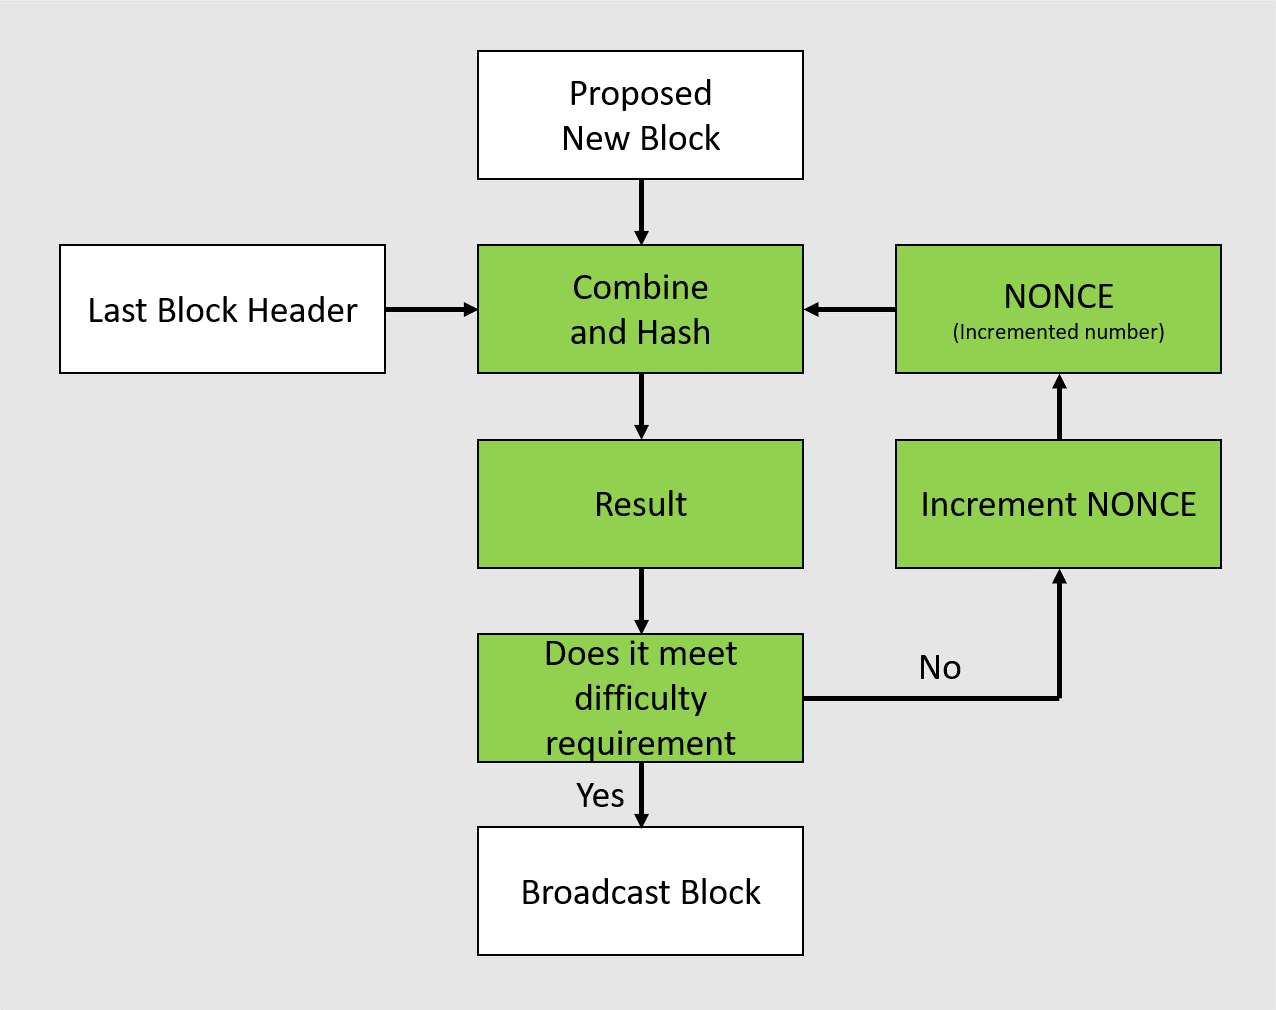
\includegraphics[width=12cm]{figures/process_to_modify.png}}}%
  \qquad
  %\caption{Cálculo de $P+Q=R$}
  %\caption{Cálculo de $2P$ y $-P$}
	\label{fig:flux}%
\end{figure}

La dificultad del puzzle, es decir, la condición que se le pide al valor hash del bloque para ser aceptado, en general no se mantiene fija. Cada determinado número de bloques (fijado en el protocolo) se vuelve a calcular este valor usando cierta función dependiente de la dificultad actual del puzzle. De esta forma según crece la cadena es necesario invertir más recursos en añadir un nuevo bloque.
% Crear un tkinter en python donde se pueden hacer pruebas e incluirlo en el apéndice.

\section{Escalabilidad del blockchain}
Aunque a medida que crece la cadena de bloques el algoritmo de prueba de trabajo garantiza una mayor resistencia a posibles ataques, surgen nuevos problemas al aumentar el número de participantes activos en la red.

Por un lado, se tiene que el tamaño máximo de cada bloque (establecido en el protocolo), es una limitación al número de transacciones que se pueden almacenar en cada ejecución del algoritmo de prueba de trabajo. A mayor números de participantes mayor será el número de operaciones y por tanto es más probable que surjan \textit{cuellos de botellas} con transacciones que deben esperar mucho tiempo por ser incluidas en la cadena.

Esto afecta fundamentalmente a la posibilidad de las criptomonedas de convertirse en alternativas serias a los métodos de pago digitales centralizados. Visa, por ejemplo, puede procesar unos 24000 pagos por segundo, mientras que criptomonedas como Ethereum o Bitcoin están limitadas a apenas 20 transacciones por segundo.\citep{scalability}

Una solución parcial a este problema ha sido aumentar el tamaño límite de los bloques admitidos en la cadena para poder almacenar más operaciones en cada ejecución del algoritmo de prueba de trabajo. Sin embargo, esta clase de cambios en el protocolo deben ser primero aceptadas por todos (o al menos buena parte) de los participantes para ser efectivas. Esto es lo que se conoce como bifurcaciones del protocolo y se analizará en la sección \ref{cap3:bifurcaciones}

\section{Uso de GPUs} %cambiar a hardware o algo asi
El algoritmo de prueba de trabajo visto en \ref{chap3:pow} se puede implementar usando computación paralela. De hecho esta es en general la forma óptima\citep{paralel_gpu} de implementarlo, pues cada procesador se encarga por separado de analizar cierto grupo de posibles valores para encontrar la solución del puzzle. Las unidades de procesamiento gráfico o GPU por sus siglas en inglés (Graphic Processing Unit) están dotadas de un mayor numero de unidades aritmético-lógicas así como de hilos de proceso, por este motivo resultan mucho mas efectivas en comparación con las CPU para realizar el minado. En los supuestos en los que se han tomado medidas en el algoritmo de consenso para evitar el uso de hardware especifico de minado se convierten en la opción mas efectiva.


Esto, por otro lado contribuyó el aumento de la demanda y por lo tanto del precio de las tarjetas gráficas\citep{gpu_price}
Una alternativa a las GPUs es el uso de circuitos integrados de aplicación específica o ASIC por sus siglas en inglés (application-specific integrated circuit). Se trata de circuitos integrados diseñados para realizar cierta tarea específica \citep{asic_def}, en el caso de las criptomonedas esta tarea es resolver la implementación del algoritmo de prueba de trabajo utilizado. Existen sin embargo variantes del algoritmo de prueba de trabajo que introducen cierta resistencia tanto al minado a través de ASIC como mediante GPU \citep{asic_res}.

\section{Resistencia a ASIC} \label{cap3:asic}

Con el aumento en la popularidad del Bitcoin, y de otras criptomonedas similares, se generalizó el uso de hardware dedicado exclusivamente al minado, es decir, a resolver el problema planteado por el algoritmo de prueba de trabajo visto en \ref{chap3:pow}. El desarrollo de esta clase de hardware ha hecho que resulte prácticamente imposible utilizar ordenadores de uso doméstico durante el proceso de minado, lo que llevado a múltiples usuarios a dejar de participar en el proceso de creación y validación de la cadena de bloques, delegando en terceros este proceso. Esta delegación de la confianza en una tercera entidad va en contra de los principios fundamentales del Blockchain. Se tienen entonces dos problemas fundamentales: por un lado el desarrollo de hardware especifico que en la práctica excluye a una parte de los usuarios de participar en el algoritmo de prueba de trabajo, por otro lado, este algoritmo hace posible delegar en otra entidad (los llamados mineros) el proceso de creación de nuevos bloques en la cadena, haciendo que parte de los usuarios no participen activamente en el proceso.
\begin{figure}[H]
%\centering
  \subfloat[Ejemplo de dispositivo ASIC (Fuente: amazon.com)]{{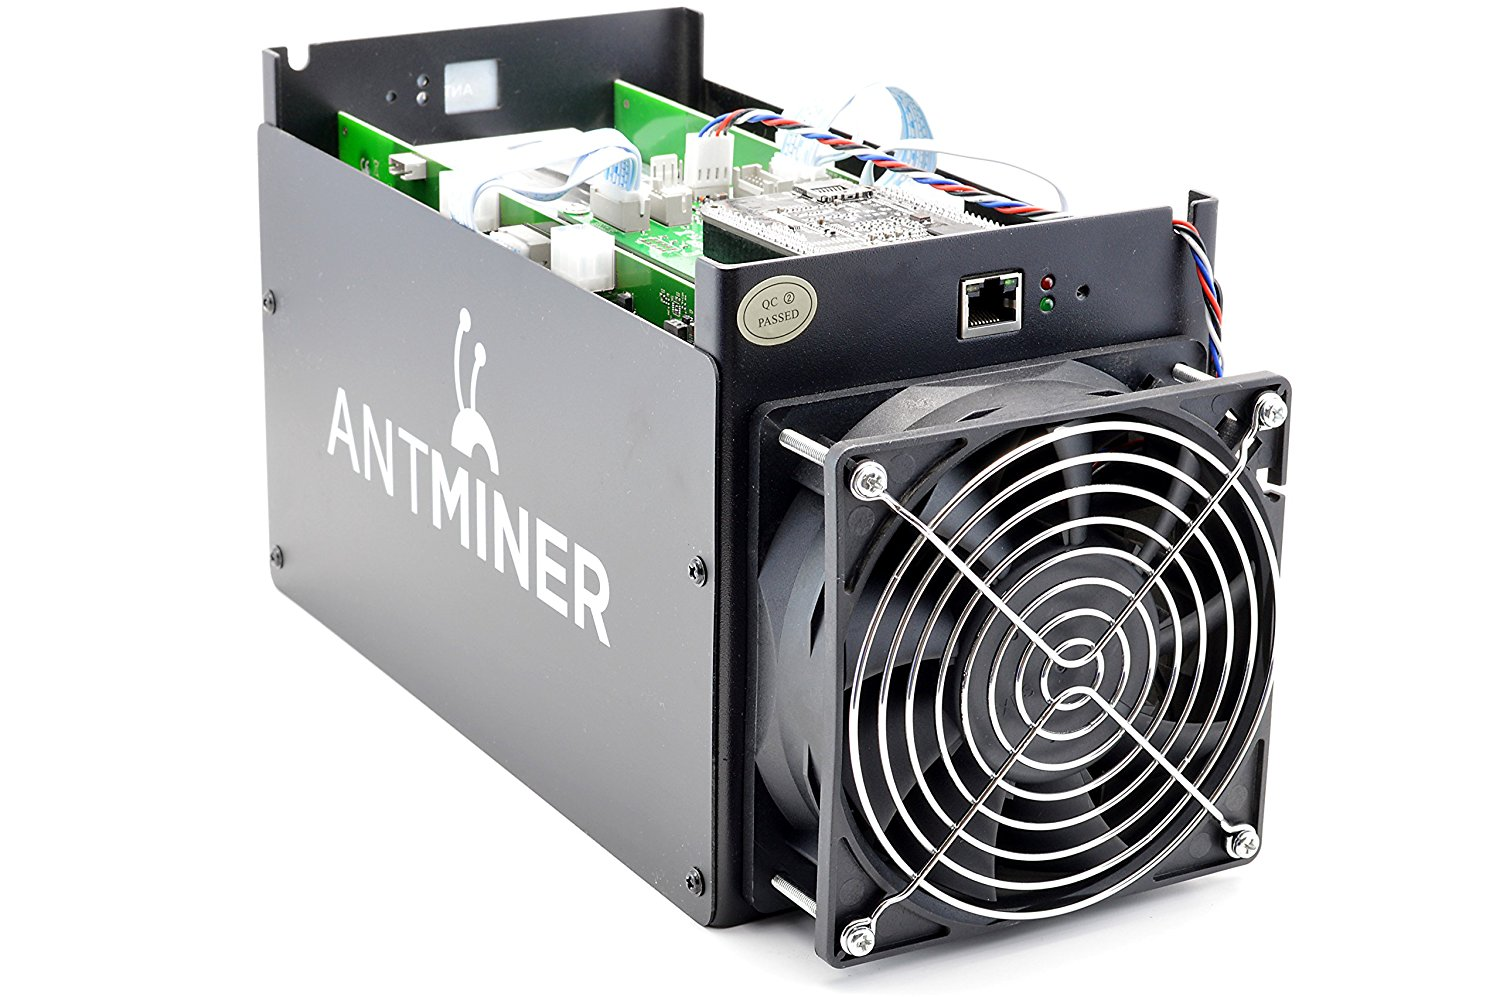
\includegraphics[width=12cm]{figures/asic.jpg}}}%
  \qquad
  %\caption{Cálculo de $P+Q=R$}
  %\caption{Cálculo de $2P$ y $-P$}
	\label{fig:test}%
\end{figure}
Estos son los motivos del desarrollo de algoritmos resistentes al minado mediante ASIC’S y que a su vez intentan minimizar la creación de nodos dedicados exclusivamente a este proceso, como las llamadas mining pools del Bitcoin. Uno de los principales algoritmos cuyo objetivo es combatir estos problemas es Hashimoto \citep{dryjahashimoto}. Se trata de un algoritmo basado en E/S, otros algoritmos creados para este fin se basaban por ejemplo en el mayor uso de memoria, pero para estos ha ido surgiendo hardware específico.

 La idea base detrás de Hashimoto no es hacer un algoritmo que sea resistente a ASIC, sino un algoritmo que funcione de forma óptima en ordenadores de uso doméstico, basado en el hecho que los límites de lectura-escritura son un problema estudiado durante años en el campo de la computación y es poco probable que el minado de monedas produzca avances significativos en esta área, y en caso de producirlos su trascendencia seria tal que impactarían en la industria del hardware en general.
Tanto en el caso de del algoritmo Hashimoto, como en el algoritmo de prueba de trabajo visto en \ref{chap3:pow} un valor hash correcto es aquel que cumple que su longitud es menor que cierto valor dado, es decir, que el valor hash empieza por n-ceros.

Este valor hash resulta de aplicar cierta función hash (SHA-256 en el caso del Bitcoin) al bloque anterior, raíz Merkle y cierto nonce. La raíz Merkle como se vio en \label{merkle} está basada en las transacciones del bloque que se quiere incluir. 


Hasta este punto Hashimoto y el método de prueba de trabajo visto antes coinciden. En lugar de detenerse en el valor hash obtenido hasta este momento en Hashimoto se realiza un segundo procesado de los datos. El conjunto de transacciones almacenados en la cadena de bloques puede considerarse ordenado. Por ejemplo la transacción número 10 del bloque 11 , podría tener el índice numero 560. Lo que hace ahora Hashimoto es acceder a diferentes puntos de la cadena, basándose en el orden anterior y en el valor hash calculado originalmente. El numero de transacciones de la cadena a las que accede es un numero fijado por el algoritmo. Se tiene entonces un conjunto de operaciones extraídas de diferentes puntos de la cadena de bloques para las que se calcula su valor hash.


El resultado (solución del algoritmo de prueba de trabajo) sera el nonce que resuelva el algoritmo de prueba de trabajo para esta combinación de valores. Así, se tiene que Hashimoto depende de acceder a casi la totalidad de la cadena de bloques. Para cadenas de bloques pequeñas esto no es un problema, pues pueden tenerse en memoria. Pero cuando estas cadenas deben mantenerse en disco por su longitud, es entonces cuando se aprecia el efecto de los tiempos de acceso de E/S. Además, se obliga a los participantes a tener una copia completa de la cadena de bloques, de otra forma dependen de la respuesta de otros nodos que almacenen el bloque para el cual quieren consultar cierta transacción. 

El algoritmo Etash, usado actualmente en la criptomoneda Ethereum está basado en Hashimoto. Este algoritmo busca 4 objetivos fundamentales \citep{etash}:
\begin{itemize}
    \item \textit{Saturar E/S} Debe forzarse el uso de casi toda la memoria RAM, basándose en el hecho que el tamano de RAM en los ordenadores de uso domestico, particularmente en las GPU's se encuentra por encima de los disponibles en dispositivos ASIC
    \item \textit{Funcionamiento optimo en GPU's} Se busca que el minado mediante GPU's sea lo mas facil posible, dado que optimizar este minado en CPU's 
    \item \textit{Fácilmente verificable} Cualquier participante debe ser capaz de verificar en un tiempo razonable una nuevo bloque.
    \item \textit{Favorecer a los clientes que almacenan la totalidad de la cadena} Aquellos que dedican espacio de almacenamiento propio para guardar la cadena de bloques tendran tiempos de acceso menores a los diferentes bloques y por tanto cierta ventaja.
\end{itemize}


\section{Bifurcaciones}\label{cap3:bifurcaciones}
Cuando se envían por la red varias versiones correctas del siguiente bloque los nodos pueden recibirlas en diferente orden. Por protocolo incluirán la primera que han recibido, así que puede ocurrir que la cadena de bloques deje de ser única. Para resolver este problema cada nodo almacena las otras versiones del último bloque que ha recibido, aunque solo considere como buena una de ellas. Con el cálculo de un nuevo bloque alguna versión se hará mas extensa que las otras (tendrá un bloque nuevo) y en este caso todos los nodos que estuvieran en una rama distinta de la cadena cambiarán a la versión más larga.

Hay que señalar que el término bifurcación (\textit{fork}) es usado también en la literatura sobre el blockchain para designar el proceso en el que se produce una modificación del protocolo acordada (o no) por los participantes. Cuando esto ocurre quienes siguen trabajando con una versión anterior dejan de reconocer los mensajes que se producen la nueva. Los que participan en este cambio pueden o bien dejar de reconocer también al protocolo antiguo y se dice entonces que estamos ante una bifurcación dura (\textit{hard fork}) o seguir aceptando estos mensajes y se dice entonces que se ha producido una bifurcación suave (\textit{soft fork}). Con esto se busca corregir errores en el código, prevenir ataques a la cadena de bloque o simplemente introducir mejoras. La resistencia a ASIC vista en \ref{cap3:asic} en caso de no existir originalmente en el protocolo, puede ser introducida posteriormente por esta vía.

%La resistencia a ASIC introducida en la criptomoneda ethereum, así como sucesivas transformaciones 
%poner ejemplo del bitcoin y del ethereum, hablar de como con esto se previene la creacion de hardware de minado especifico para determinado protocolo, hablar también de bifurcaciones accidentales
%\section{Árboles Merkle}

%definir y explicar como se usan
\section{Alternativas a la prueba de trabajo}
El método de prueba de trabajo explicado en \ref{chap3:pow} al estar basado en la realización de un gran número de operaciones, ya sea en CPU, GPU o ASIC tiene ciertos inconvenientes. Por un lado, entidades con el poder suficiente para controlar un gran número de máquinas pueden intentar alterar el protocolo de consenso en la red. Como vimos esto se intenta solucionar, al menos parcialmente, al introducir medidas contra el minado usando hardware específico, permitiendo de esta forma que los usuarios domésticos participen en igualdad de condiciones. Pero nada impide que ciertas entidades utilicen gran numero de CPU's o GPU's para intentar hacer modificaciones en la cadena de bloques.
En general la filosofía del Blockchain supone que alguien que tiene interés en participar en el protocolo y lo demuestra invirtiendo su tiempo de procesamiento estará también interesado en que el consenso se mantenga y por tanto no validará operaciones falsas. Igualmente, se pueden utilizar las bifurcaciones explicadas en \ref{cap3:bifurcaciones} para modificar el protocolo si es necesario contrarrestar algún tipo de hardware específico diseñado para hacer más efectivo el proceso de minado.
 %(en el enlace \url{goo.gl/xn4D5s} se puede ver un ejemplo de esto).url https://ethereumworldnews.com/ethereum-hard-fork-proposed-in-response-to-new-asic-miners/

Otra de las consecuencias negativas del protocolo de prueba de trabajo es de índole ecológica. El coste computacional de una red grande, como la de las criptomonedas Bitcoin y Ethereum por ejemplo, se refleja en un gasto energético extraordinario. Hay que tener en cuenta que en el proceso de validar un conjunto de operaciones solo se tiene en cuenta el resultado del primero que resuelve el puzzle, y por tanto el trabajo de todos los que han estado trabajando en ese mismo bloque ha sido en vano. Se estima que la red del Bitcoin a finales de 2017 ya gastaba más energía eléctrica que 159 países \citep{electricidad}. Teniendo en cuenta que las principales fuentes energéticas continúan siendo los combustibles fósiles es comprensible la preocupación que esto despierta.

A la vista de lo anterior se han propuesto varias alternativas entre las que se destacan las siguientes:
\begin{itemize}
\item \textit{Prueba de participación (Proof of Stake)}: Para validar las transacciones se hace necesario disponer de cierta cantidad del recurso en que se basa la red (generalmente criptomonedas). En base a la cantidad de este recurso que posea, cada participante tiene asignado un peso que representa el valor de sus decisiones (a mayor cantidad de recursos mayor poder de decisión). Para proponer y elegir el siguiente bloque de la cadena se tienen en cuenta los votos y propuestas de cada participante de acuerdo a su peso. La filosofía detrás de esta idea es que quienes posean un mayor número del recurso de la red estarán más comprometidos con ella y por tanto serán los mejores garantes del consenso. Este método se puede combinar con la prueba de trabajo para de esta forma reducir la complejidad del puzzle que hay que resolver, o implementarlo de forma independiente. En ambos casos representa un notable ahorro energético respecto a la prueba de trabajo.

Por otro lado, se tiene el problema de cómo iniciar la cadena cuando ninguno de los participantes posee recurso alguno. Debido a esto, se suele optar por un enfoque mixto entre ambos métodos. Ejemplos del uso de este método están en versiones más recientes de Ethereum y en la criptomoneda Peercoin \citep{pos}

\item \textit{Proof of burn:} En este caso para obtener el derecho de validar transacciones (crear bloques) hay que destruir cierto recurso como prueba de nuestro compromiso con la red. Generalmente el recurso que se destruye es otra criptomoneda y esto se consigue enviándola a determinada dirección desde donde es irrecuperable. Este método tiene el problema de requerir de la existencia de al menos una moneda con ciertas propiedades similares a la nuestra (si es fácil crearla por ejemplo no tiene valor práctico destruirla). Aunque este mecanismo no requiera de un gran consumo energético la moneda alternativa que estamos destruyendo puede que esté basada en la prueba de trabajo, así que estaríamos en una situación similar a la explicada al inicio de este sección. Por todo esto la aplicación de este método aunque interesante desde el punto de vista económico, resulta contraproducente respecto al problema del gasto energético. 

La criptomoneda Slimcoin es la primera implementación de este algoritmo de consenso \citep{pob}
\end{itemize}

%.. alternativas: proof of stake, proof of capacity, proof of burn... Todas estas alternativas siguen dependiendo del PoW, solo que reducen el coste computacional al imponer nuevas condiciones.


\section{Privacidad y seguridad}\label{cap3:seguridad} %correccion??
Al inicio de este capítulo se explicaron los objetivos del Bitcoin, sin embargo, no se hizo referencia a la privacidad. En los sistemas bancarios tradicionales se mantiene cierto nivel de confidencialidad, y por tanto la información sobre el balance y las operaciones de determinada cuenta no se comparten libremente. En un sistema basado en el blockchain surge el problema de como garantizar la privacidad en un entorno público donde las transacciones por definición deben ser vistas por todos los participantes. Esto se resuelve manteniendo en secreto la identidad de los poseedores de las  claves públicas. Además si se usa una clave pública distinta en cada transacción incluso aunque se llegue a comprometer la privacidad de alguna de nuestras claves se siguen manteniendo ocultas las otras y en consecuencia es imposible que alguien llegue a conocer todas las operaciones que hayamos realizado y nuestro balance total. 

En este sentido los sistemas monetarios basados en blockchain guardan cierta semejanza con el dinero físico y se hace necesario disponer de algún sitio seguro donde guardar el conjunto de claves privadas que hayamos usado ya sea para recibir transferencias o recompensas por haber participado en el algoritmo de consenso. Estos son los llamados monederos (wallets), que existen tanto en forma de software como de hardware específico.
Estas cuestiones sobre privacidad aunque en las criptomonedas se consideran necesarias no son imprescindibles y en otras aplicaciones del blockchain se pueden obviar.


Otra cuestión de gran relevancia es como de segura es una red basada en blockchain. Por un lado, hay que distinguir aquellos ataques basados en intentar encontrar la clave (o claves) privada de un usuario  y por otro los ataques al protocolo de consenso de la red. En el primer caso, la seguridad de la red depende en gran medida de la implementación del algoritmo visto en \ref{cap1}. Sobre el problema del logaritmo discreto para curvas elípticas (en el que se basa el ECDSA) no se conoce ningún algoritmo que lo resuelva en tiempo subexponencial \citep{discrete_log}. Por tanto, se puede considerar que encontrar la clave privada a partir de la pública es infactible siempre que se haya implementado correctamente el algoritmo de cifrado. Evidentemente es igual de importante almacenar las claves privadas en un sitio seguro.
Los ataques al protocolo de consenso se basan en intentar que sean incluidos en la cadena bloques con información falsa, en el caso de las criptomonedas esto es el problema del doble gasto mencionado al inicio de este capítulo. Por ser este un problema de gran interés dentro de la programación distribuida y que va más allá de la idea de blockchain se tratará en el siguiente capítulo con más detalle.  %donde un nodo malicioso intenta usar más dinero del que realmente posee. En e% Para la función hash SHA-256 como se dijo en \ref{hash} no se conocen colisiones hasta la fecha, así que un posible atacante no podría aprovecharse de esta clase de vulnerabilidades y debería por tanto usar el algoritmo de prueba de trabajo en igualdad de condiciones con los otros participantes.